% !TEX root = ../main.tex
\chapter{The PFASST method}
\label{chapter:pfasst}

\section{Deferred correction}

The definitions in this section are summarized from \cite{dutt2000spectral}, where detailed derivations for each method and in-depth observations may be found.

For an initial value problem in the standard form
\begin{gather}
    u'(t)=f(t,u(t)),\quad t\in[a,b], \label{eq:ivp} \\
    u(a)=u_a \nonumber
\end{gather}
where \(u_a,u(t)\in\mathbb{C}^n\) and \(f \colon \mathbb{R} \times \mathbb{C}^n \to \mathbb{C}^n \), we can integrate \ref{eq:ivp} with respect to \(t\) to obtain the equivalent Picard equation
\begin{equation}
    u(t)=u_a + \int_a^t f(\tau,u(\tau))d\tau.
	\label{eq:picard_ivp}
\end{equation}

Given an approximate solution \(\tilde{u}(t) \approx u(t)\) to \ref{eq:picard_ivp}, its quality can be measured by the residual function
\begin{equation}
    \varepsilon(t,\tilde{u}(t)) = u_a + \int_a^t f(s,\tilde{u}(s))ds - \tilde{u}(t).
	\label{eq:residual}
\end{equation}

Defining the error \(\delta(t)\) by
\begin{equation}
    \delta(t) \coloneqq u(t)-\tilde{u}(t),
	\label{eq:error}
\end{equation}
we can substitute \ref{eq:error} into \ref{eq:picard_ivp}, and, through algebraic manipulation, arrive at
\begin{equation}
    \delta(t) = \int_a^t (
    f(\tau,\tilde{u}(\tau)+\delta(\tau)) 
    - f(\tau,\tilde{u}(\tau))) d\tau
    + \varepsilon(t,\tilde{u}(t))
    \label{eq:dcmethod_ivp}
\end{equation}
which is a Picard-type integral in the same form as \ref{eq:picard_ivp}.

Supposing we wish to solve the IVP from and \ref{eq:ivp} in an equispaced grid of \( m+1 \) nodes defined by
\begin{equation}
    t_i = a + i \cdot h, \quad i = 0,\ldots,m,
\end{equation}
with step size \( h=(b-a)/m \). A method of \(k\)-th order accuracy by definition yields an approximate solution \( \tilde{u} = \tilde{u}_1, \ldots, \tilde{u}_m \) with
\begin{equation}
    \tilde{u}_i = u(t_i)+O(h^k).
    \label{eq:approx_sol_accuracy}
\end{equation}

This approximate solution can be interpolated at the grid points \(t_i\) by the unique \(m\)-th order Lagrange polynomial \(u_p(\eta,t)\). This allows the definition of an error function analog to \ref{eq:error}
\begin{equation}
    \delta(t) \coloneqq u(t)-u_p(\tilde{u},t),
	\label{eq:interp_error}
\end{equation}
which satisfies the IVP
\begin{gather}
    \delta'(t) = f(t,\delta(t) + u_p(\tilde{u},t)) - \frac{d}{dt}u_p(\tilde{u},t) \label{eq:error_ivp}\\ 
    \delta(0) = 0. \nonumber
\end{gather}

Equation \ref{eq:error_ivp} can then be solved for using the same \(k\)-th order method as the original problem, generating an approximation for the error \(\pi_i \approx \delta(t_i)\). This approximation can then be to correct \(\tilde{u}\)
\begin{equation}
    \tilde{u}_i + \pi_i \approx y(t_i),
	\label{eq:dc_correction}
\end{equation}
where the corrected solution is of \(2k\)-th order accuracy. This method can then be further iterated by computing a new interpolating polynomial for the updated solution, defining a new error function, and solving the IVP in \ref{eq:error_ivp} to obtain a new estimated error.

After \(J\) iterations, the error of the approximate solution \(\varphi^J(t)\) is of the order \cite{dutt2000spectral} 
\begin{equation}
    O(h^{(J+1) \cdot k}).
	\label{eq:dc_error}
\end{equation}

\section{Spectral deferred correction} \label{sec:math_sdc}

Spectral deferred correction improves on classical deferred correction though the use of quadrature rules that enable robust numerical integration over the interval of interest. Note that while SDC was originally proposed in \cite{dutt2000spectral} using Gauss-Legendre nodes, it is commonly employed using different quadrature rules, such as Gauss-Lobatto and Gauss-Radau. A detailed analysis of the implications of quadrature choices for SDC can be found in \cite{layton2005implications}. This section was adapted from from \cite{speck2015multi}.

We define \(t \coloneqq (t_i)\) as the nodes in the chosen quadrature in the interval \([a,b]\), with \(a = t_0 < t_1 < \ldots < t_M = b\), and \(U_j = u_p(t_j) \approx u(t_j)\), where \(u_p\) is the collocation polynomial in \([a,b]\). We also define \(q\) as the matrix of quadrature weights with elements

\begin{equation}
    q_{m,j} \coloneqq
    \frac{1}{\Delta t}
    \int^{t_m}_a l_j(s)ds, \quad m,j=0,\ldots,M,
    \label{eq:quadrature_q}
\end{equation}

where \(l_j\) are the Lagrange polynomials defined by \(t\) and \(\Delta t=b-a\). Noting that the quadrature in \refEquation{eq:quadrature_q} interpolates \(u_p\) exactly, we can insert \refEquation{eq:quadrature_q} in \refEquation{eq:picard_ivp} to obtain

\begin{equation}
    U_m = u_0 + \Delta t 
    \sum_{j=0}^M q_{m,j} f(U_j, t_j), \quad m=0,\ldots,M
    \label{eq:sdc_element}
\end{equation},

and the residual \(\varepsilon(t_j,U_j)\) can be computed by

\begin{equation}
    \varepsilon(t_j,U_j) = u_0 + \Delta t 
    \sum_{j=0}^M q_{m,j} f(U_j, t_j) - U_j, \quad m=0,\ldots,M
    \label{eq:sdc_element_residual}
\end{equation}.

Using the residual obtained in \refEquation{eq:sdc_element_residual}, \refEquation{eq:dcmethod_ivp} can be solved through the desired scheme, obtaining an approximate error that can be used to correct the current solution like in classical deferred correction. This SDC iteration shown above is also referred to in the context of PFASST as a \textit{sweep}, and the method used in the solution of the error estimate as a \textit{sweeper}.

This method has numerical advantages over the classical deferred correction scheme. The choice of non-equispaced nodes avoids the occurrence of Runge's phenomenon, and the resulting integration matrix is numerically well-conditioned \cite{dutt2000spectral}.

\section{Full approximation scheme} \label{sec:fas}

The \textit{full approximation scheme} (FAS) is a multigrid scheme commonly used for nonlinear problems. Its name derives from solving the coarse-grid problem for an approximation of the fine-level solution, instead of only the error as is standard for linear multigrid methods. 

Here, let's denote the problem on level \(\ell\) by
\begin{equation}
    A_\ell(u_\ell)=f_\ell,
    \label{eq:fas_l_eq}
\end{equation}
the approximate solution on that level by \(v_\ell\), and the interpolation and restriction operators, respectively, by \(I\) and \(R\). A two level FAS scheme for this problem is described as follows \cite{briggs2000multigrid}:

\begin{enumerate}
    \item Restrict the current approximation and its fine-grid residual to the coarse grid: \(r_2 = R(f_1 - A_1(v_1))\) and \(v_2 = R v_1\).
    \item \label{fas_coarse_step} Solve the coarse-grid problem \(A_2(u_2) = A_2(v_2) + r_2\).
    \item Compute the coarse-grid approximation to the error: \(e_2 = u_2 - v_2\).
    \item Interpolate the error approximation up to the fine grid and correct the current fine-grid approximation: \(v_1 = v_1 + Ie_2\)
\end{enumerate}

The equation for the coarse grid in \ref{fas_coarse_step} can alternatively be written as

\begin{equation}
    A_{\ell+1}(u_{\ell+1})=f_{\ell+1}+\tau_{\ell+1}
    \label{eq:fas_lp1_eq}
\end{equation}

where the correction term \(\tau_{\ell+1}\) is defined by

\begin{equation}
    \tau_{\ell+1}=A_{\ell+1}(Rv_{\ell})-RA_\ell(v_\ell).
    \label{eq:fas_tau}
\end{equation}

Using this, we can rewrite the FAS scheme in the form:

\begin{enumerate}
    \item Restrict the current approximation to the coarse grid: \(v_2 = R v_1\)
    \item Compute the correction term \(\tau_2\) using \refEquation{eq:fas_tau}.
    \item Solve the coarse-grid problem \(A_2(u_2)=f_2+\tau_2\)
    \item Compute the coarse-grid approximation to the error: \(e_2 = u_2 - v_2\).
    \item Interpolate the error approximation up to the fine grid and correct the current fine-grid approximation: \(v_1 = v_1 + Ie_2\)
\end{enumerate}

\section{Parareal}

Parallelization of the solution of PDEs in the spatial dimensions, including but not limited to the previously described methods, is a well-established field of research. However, for a fixed problem size, Amdahl's law dictates a limit for the parallel speedup with an increasing number of processors. As many high-performance applications reach this saturation point, parallelization in the time dimension becomes increasingly attractive. Though the theoretical foundations for it were established over half a century ago, parallelization in time remains a relatively small field of research \cite{dongarra2014applied}. While standard time integration methods sequentially iterate through time steps, parallel-in-time methods use an approach similar to deferred correction methods, computing an approximate solution over the full domain and iteratively refining it.

For an IVP of the form \ref{eq:ivp}, the Parareal method for parallelization across \(N\) processors is constructed \cite{ruprecht2014convergence}\cite{gander2007analysis} by partitioning the time domain into slices \([t_{n-1}, t_n], n = 1,\dots,N\), where \(t_0 \coloneqq a < t_1 < \dots < t_N \coloneqq b\) . Let \(\mathcal{F}(u_n, t_{n+1}, t_n)\) (also referred to in the context of Parareal as the \textit{fine propagator}) be an operator providing a sufficiently accurate approximation to \(u(t_{n+1})\) for the initial condition \(u(t_n)=u_n\) (e.g. a higher-order Runge-Kutta method). Serial integration of \ref{eq:ivp} using \(\mathcal{F}\) is equivalent, with \(u_0 \coloneqq u_a\), to evaluating

\begin{equation}
    u_{n+1} = \mathcal{F}_{\delta t}(u_n, t_{n+1}, t_n), \quad n = 0,\dots,N-1.
    \label{eq:parareal_seq}
\end{equation}

Now let \(\mathcal{G}\), the \textit{coarse propagator}, be an operator providing a rougher approximation of \(u(t_{n+1})\), typically a lower-order method with higher time step size. Given an initial approximate solution \(u_n^0, n = n = 0,\dots,N\), the Parareal algorithm performs corrective iterations of the form

\begin{equation}
    u^{k+1}_{n+1} = \mathcal{G}(u^{k+1}_n, t_{n+1}, t_n) + \mathcal{F}(u^k_n, t_{n+1}, t_n) + \mathcal{G}(u^k_n, t_{n+1}, t_n).
    \label{eq:parareal_it}
\end{equation}

Parallelization of each iteration is achieved by sequential computation of the coarse propagator \(\mathcal{G}\), followed by parallel computation of the fine propagator \(\mathcal{F}\). As detailed in \cite{gander2007analysis}, this iteration is equivalent to a two-level multigrid FAS iteration (as described in \refSection{sec:fas}) in the time domain.

After \(k\) iterations, the solution \(u_n^k, n \leq k\) is exactly equal to the one obtained for \(u_n\) in \ref{eq:parareal_seq}. Hence, after \(N\) iterations, the Parareal method is guaranteed to match the serial solution, but in practice it converges more quickly for large \(N\). Since Parareal adds the computational cost of \(\mathcal{G}\) and the communication overhead, it can only provide speedup compared to serial execution if the number of iterations required for convergence is significantly less than \(N\). By assuming the time slices to be uniform (\(t_N - t_{N-1} = \dots = t_1 - t_0\), and their size to be a multiple of the constant time steps of \(\mathcal{F}\) and \(\mathcal{G}\), it can be shown that the parallel efficiency of Parareal is bounded by \(1/K\), where \(K\) is the number of iterations needed for convergence. \cite{minion2011hybrid}

\section{PFASST}

The \textit{parallel full approximation scheme in space and time} (PFASST), presented in \cite{emmett2012toward}, can be thought of as a modification of Parareal in the following aspects:

\begin{itemize}
    \item Rather than a direct solution, the fine propagator consists of one or more SDC sweeps. Additionally, for an iteration \(k\), its initial condition is not \(u^k_n\) as in Parareal, but instead the approximate solution obtained from iteration \(k-1\) for the time slice, significantly lowering the number of SDC sweeps needed;
    \item The coarse propagator also consists of SDC sweeps, operating on a coarsened grid in time and space dimensions. FAS correction is applied to these sweeps, allowing the coarse propagator to achieve the accuracy of the fine propagator at the resolution of the coarse grid;
    \item During initialization, processors do not idly wait for an initial condition from the previous processor, but instead start their own coarse sweeps during this time, with processor \(P_n\) performing \(n\) iterations of the coarse propagator during this stage. This significantly improves solution accuracy without impacting total execution time.
\end{itemize}

Like Parareal, PFASST partitions the time domain of a problem of the form \ref{eq:ivp} into \(N\) uniform slices, with \([t_n, t_{n+1}]\) being assigned to processor \(P_n, n = 1,\dots,N-1\). Each slice is further divided into \(M+1\) fine SDC nodes \(t_{n,0} \coloneqq t_n < \dots < t_{n,M} \coloneqq t_{n+1}\), and \(\tilde{M}+1\) fine SDC nodes \(\tilde{t}_{n,0} \coloneqq t_n < \dots < \tilde{t}_{n,\tilde{M}} \coloneqq t_{n+1}\). For iteration \(k\) and processor \(P_n\), we denote the approximate solution at the \(m\)-th fine node by \(u^k_{n,m}\) and at the \(\tilde{m}\)-th coarse node by  \(u^k_{n,\tilde{m}}\). Additionally, let

\begin{equation}
    \bm{u}^k_n \coloneqq 
    \begin{bmatrix}
        u^k_{n,1} \\ \vdots \\ u^k_{n,M} % yes, u and f have different dimensions
    \end{bmatrix}
    \quad \text{and} \quad
    \bm{f}^k_n \coloneqq
    \begin{bmatrix}
        f(t_{n,0}, u^k_{n,0}) \\ \vdots \\ f(t_{n,M}, u^k_{n,M})
    \end{bmatrix}
\end{equation},

with analogous notation for the coarse level. During initialization, we denote as \(\bm{\tilde{u}}^{0,j}_n\) and \(\bm{\tilde{f}}^{0,j}_n\) the values for the \(j\)-th iteration of the coarse propagator.

PFASST execution starts by spreading the initial solution \(u(a)\) to all fine SDC nodes \(\bm{u}^0_n\), after which execution at processor \(P_n\) proceeds as below:

\begin{enumerate}
    \item \textbf{Initialization:} Set all \(\bm{u}^0_n\) = \(u(0)\), evaluate \(\bm{f}^0_n\).
    \item Restrict \(\bm{u}^0_n\) to \(\bm{\tilde{u}}^{0,0}_n\), evaluate \(\bm{\tilde{f}}^{0,0}_n\).
    \item Compute FAS correction between \(\bm{f}^0_n\) and \(\bm{\tilde{f}}^{0,0}_n\), yielding \(\bm{\tau}^0_n\).
    \item For \(j = 0, \dots, n-1\):
        \begin{enumerate}    
            \item If \(n > 0\) and \(j > 0\): receive \(\tilde{u}^{0,j}_{n,0}=\tilde{u}^{0,j}_{n-1,\tilde{M}}\) from \(P_{n-1}\)
            \item Perform coarse SDC sweeps with \(\bm{\tilde{u}}^{0,j-1}_{n}\), \(\bm{\tilde{f}}^{0,j-1}_n\) and \(\bm{\tau}^0_n\), yielding \(\bm{\tilde{u}}^{0,j+1}_{n}\) and \(\bm{\tilde{f}}^{0,j+1}_n\)
            \item If \(n < N-1\): send \(\tilde{u}^{0,j+1}_{n,\tilde{M}}\) to \(P_{n+1}\)
        \end{enumerate}
    \item Set \(\bm{\tilde{u}}^{0}_{n}\) to \(\bm{\tilde{u}}^{0,n}_{n}\)\)% evaluate \(\bm{\tilde{f}}^{0}_{n}\). removed because value isn't used
    \item Interpolate coarse correction \(\bm{\tilde{u}}^{0,n}_{n} - \bm{\tilde{u}}^{0,0}_{n}\), yielding \(\bm{u}^{0}_{n}\). Evaluate \(\bm{f}^{0}_{n}\).
    \item \textbf{PFASST iterations:} For \(k = 1, \dots, K\):
        \begin{enumerate}
            \item Perform fine SDC sweeps with \(\bm{u}^{k-1}_{n}\) and \(\bm{f}^{k-1}_{n}\), yielding \(\bm{u}^{k}_{n}\) and \(\bm{f}^{k}_{n}\)
            \item Restrict \(\bm{u}^{k}_{n}\) to \(\bm{\tilde{u}}^{k}_{n}\), evaluate \(\bm{\tilde{f}}^{k}_{n}\)
            \item Compute FAS correction \(\bm{\tau}^k_n\) from \(\bm{f}^{k}_{n}\) and \(\bm{\tilde{f}}^{k}_{n}\)
            \item If \(n > 0\): receive \(u^{k}_{n,0}=u^{k}_{n-1,M}\) from \(P_{n-1}\), restrict \(u^{k}_{n,0}\) to \(\tilde{u}^{k}_{n,0}\)
            \item Perform coarse SDC sweeps with \(\bm{\tilde{u}}^{k}_{n}\), \(\bm{\tilde{f}}^{k}_{n}\) and \(\bm{\tau}^k_n\), yielding updated \(\bm{\tilde{u}}^{k}_{n}\) and \(\bm{\tilde{f}}^{k}_{n}\)
            \item Interpolate coarse correction \(\tilde{u}^{k}_{n,\tilde{M}} - \tilde{u}^{k-1}_{n,\tilde{M}}\), yielding \(u^{k}_{n,M}\)
            \item If \(n < N-1\): send \(\tilde{u}^{0,j+1}_{n,\tilde{M}}\) to \(P_{n+1}\)
            \item Interpolate coarse correction \(\tilde{u}^{k}_{n} - \tilde{u}^{k-1}_{n}\), yielding \(u^{k}_{n}\), evaluate \(f^{k}_{n}\)
        \end{enumerate}
\end{enumerate}

\begin{figure}[ht]
  \centering
  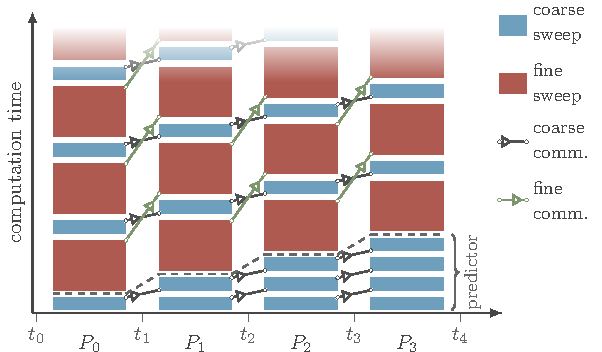
\includegraphics[width=\textwidth]{images/pfasst_diagram.pdf}
  \caption{Representation of the PFASST method using two levels. Created using pfasst-tikz\footnotemark.}
\end{figure}
% END: ensure it's on the same page as the picture
\footnotetext{\url{https://github.com/f-koehler/pfasst-tikz}}

With \(K_s\) denoting the number of SDC iterations needed to compute the solution to the desired accuracy in serial using the fine nodes, and \(K_p\) denoting the number of PFASST iterations for the same accuracy, the parallel efficiency of PFASST is bounded by \(E < K_s/K_p\). That is, when compared to standard Parareal with SDC propagators (\(E < 1/K_p\)), the bound is relaxed by a factor of \(K_s\).

\section{LibPFASST} \label{sec:libpfasst_usage}

Proper implementation of numeric methods is time-consuming and error prone. This chapter presents a simplified overview of the building blocks of the PFASST scheme, but omits the more complex mathematical aspects an implementation must account for. Additionally, parallel programs are notoriously hard to validate. These factors come together to make an efficient, reliable implementation of the PFASST method particularly hard to accomplish. For a user wanting to apply PFASST (or one of the other schemes mentioned in this section) to the solution of a specific problem, or even to implement a modified version of a method, it is better to start from a known, reliable open-source implementation.

LibPFASST \cite{libpfasst_github} is an implementation of the PFASST algorithm, written in Fortran 2008 using MPI for parallelization. It offers, through different configurations, support for all the methods previously described, as well as a number of additional variations of PFASST components which aren't mentioned here. It structured in a modular and extensible way, facilitating mixing and matching of different PFASST components and user-created components, and optionally integrates with other libraries such as PETSc, AMReX and Sundials.

Here we aim to provide a simplified introduction to the usage of LibPFASST, which will be useful in illustrating details of the cpfasst implementation. For a  complete user's guide to LibPFASST, refer to \cite{libpfasst_ug}. This description is based on the tutorial \ilc{EX2_Dahlquist}, included with the LibPFASST source code.

The usage of LibPFASST to solve a simple problem involves the steps below:

\begin{itemize}
    \item \textbf{Configure LibPFASST parameters:} LibPFASST has a few mandatory parameters, and several optional ones. These include tolerances, number of levels and sweeps per level, number and type of nodes, and several others - a comprehensive guide is provided in \cite{libpfasst_ug}. The configuration is stored in an instance of the main LibPFASST structure, \ilc{pf_pfasst_t}, and can be initialized and changed through any combination of nml file parameters, command line parameters, and writing to the \ilc{pf_pfasst_t} structure in user code.

    \item \textbf{Choose (or define) a data encapsulation:} Choose a type to represent a single instance of the solution over the space domain for one level. LibPFASST provides several such types to choose from, e.g. \ilc{pf_ndarray_t}, which implements an n-dimensional array of real numbers. Alternatively, a custom encapsulation can be implemented by the user, by extending type \ilc{pf_encap_t}, and defining its deferred type-bound procedures, which are used to operate on the encapsulated data (e.g. \ilc{norm}, \ilc{axpy}). The data encapsulation must be paired with a compatible factory to create and destroy the encapsulation type, which is provided for the predefined encapsulations, but can also be customized by the user through a type extending \ilc{pf_factory_t}.

    \item \textbf{Define a user level:} The user must define a type extending \ilc{pf_user_level_t}, and implementing its deferred type-bound procedures \ilc{restrict} and \ilc{interpolate} for the chosen encapsulation. Those are invoked by LibPFASST for the multi-level spatial restriction and interpolation operations. FAS correction is handled automatically by LibPFASST. 

    \item \textbf{Define a sweeper:} The user must define a type expanding one of the LibPFASST sweeper types, and implementing any deferred type-bound procedures contained in that sweeper. Each of the sweeper types is suitable to the solution of problems of a certain form, and these procedures are used for problem-specific evaluations in the given form. In the case of the implicit-explicit sweeper used in this project, suitable for problems of the form \(y'=f_1(y,t)+f_2(y,t)\), where \(f_1\) is treated explicitly and \(f_2\) implicitly, the procedures to be defined are:
    \begin{itemize}
        \item \ilc{f_eval}: Evaluate the requested piece of the right-hand side function (\(f_1\) or \(f_2\)) for the provided time \(t\) and approximate solution \(y\).
        \item \ilc{f_comp}: Implicitly solve the equation \(y-dtq*f_2(y,t)=rhs\) for the provided time \(t\), approximate solution \(y\), right-hand side value \(rhs\), and \(dtq\in\mathbb{R}\).
    \end{itemize}
\end{itemize}